% !TEX TS-program = xelatex
% !TEX encoding = UTF-8 Unicode

% Tennessee Technological University
% ME4140 - Fall 2016 - Fall 2017 - ? - Fall 2019 - Fall 2020
% Tristan Hill - September 19, 2020 - October 09, 2020
% Turtorial 7 - Turtlebot3 in Brown Hall 

\documentclass[12pt]{article}

% Custom Preamble
\usepackage{/home/thill/Documents/lectures/ros_workshop/ros_tutorial} 

% Title and Misc
\newcommand{\MNUM}{7} %Module Number
\newcommand{\MNAME}{Turtlebot3 in Brown Hall} %Module Name
\pagestyle{myheadings}
\markright{{\large ME4140 - ROS Workshop - Fall 2020}}

%\newcommand{\pkgname}{<package\_name>}
%\newcommand{\wspname}{<workspace\_name>}
%\newcommand{\nodname}{<node\_name>}
%\newcommand{\tpcname}{<topic\_name>}
%\newcommand{\lfname}{<file\_name>}
%\newcommand{\home}{\textasciitilde/}
%\newcommand{\rosdistro}{melodic}
%\newcommand{\pthname}{/opt/ros/\rosdistro/share/turtlebot\_stage/maps/}


\begin{document}

\thispagestyle{plain}

\begin{center}
   {\bf \Large ROS Workshop - Tutorial\hspc\MNUM\hspc - \MNAME}\vspace{3mm}\\
   {\bf \large ME 4140 - Introduction to Robotics - Fall 2020} \vspace{5mm}\\
\end{center}



What is the goal of the.  This tutorial comes from \href{http://emanual.robotis.com/docs/en/platform/turtlebot3/simulation/#simulation} {here.}  \\

%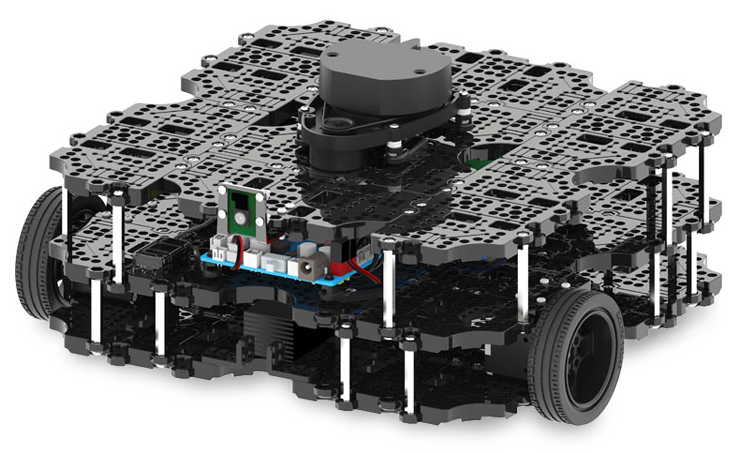
\includegraphics[scale=.25]{turtlebotPi.jpg}
%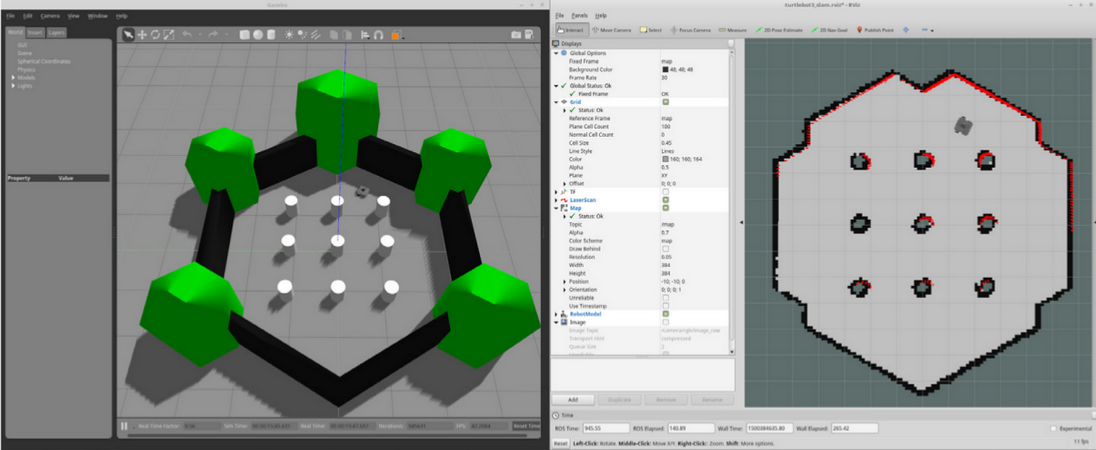
\includegraphics[scale=.3]{turtlebot3_maps.png} 

\begin{description}[labelindent=1cm]
	
	\item[\textbf{\underline{Overview:}}] \hfill \vspace{3mm}\\
	After completing {\it Tutorial 6 - Turtlebot Navigation}, You have learned some basics of ROS, and you have a for a more advanced robot. Next you are going to learn to load a custom world in Gazebo. Read more \href{http://gazebosim.org/tutorials?tut=ros_gzplugins}{here}.
	
	\item[\textbf{\underline{System Requirements:}}] \hfill \vspace{0mm}

\begin{itemize}
	\item {\bf ROS+OS}: This tutorial is intended for a system with ROS Melodic installed on the Ubuntu 18.04 LTS operating system. Alternate versions of ROS (i.e. - Kinetic, Noetic, etc.) may work but have not been tested. Versions of ROS are tied to versions of Ubuntu.
	\item {\bf ROS:} Your computer must be connected to the internet to proceed. Update the system before you begin.
	\item {\bf Workspace Setup:} The Turtlebot3 Simulator from tutorial 6 must be operational before completing tutorial 7.  
\end{itemize}

	
	\item[\textbf{\underline{Disclaimer:}}] \hfill \vspace{0mm}
	
	\begin{itemize}

		\item {\R\underline{\bf Backup the System:}} If you are using a virtual machine, it is recommend to make a snaphot of your virtual machine before you start each module. In the event of an untraceable error, you can restore to a previous snapshot. 
		
		\item \underline{\B ROSLAUNCH:} This tutorial involves using the roslaunch command which runs a muliple of nodes at once as described in the launch file. We will learn more about this later. 
	
		\item \underline{\G Mouse for 3D viewing:} This simulator view is much easier use if you have a three button mouse plugged in, but this is not required.
	
		 
	\end{itemize}
   
\newpage   
    
    \item Create a new node with the name of your choosing. You can put this node in the package you created previously for turtlebot3.  Change directory to the source folder of the package and enter the following command to open a new file for your source code.
\begin{minted}{text}
gedit |\home\wspname|/src/turtlebot3|\_|control/src/publish|\_|goal.cpp
\end{minted}

    

    \item Now copy the example code below into the the source file. Save the file after editing. \\
    
        \begin{lstlisting}
#include "ros/ros.h"
#include "geometry_msgs/PoseStamped.h"
#include <sstream>
int main(int argc, char **argv)
{
    ros::init(argc, argv, "<node_name>");
    ros::NodeHandle n;
    ros::Publisher ttu_publisher =
    n.advertise<geometry_msgs::PoseStamped>("<topic_name>", 1000);
    ros::Rate loop_rate(10);

    geometry_msgs::PoseStamped msg;
    msg.header.stamp=ros::Time::now();
    msg.header.frame_id="map";

    int count = 0;
    while ((ros::ok())&&(count<5))  
    {               
        msg.pose.position.x = 3.0;
        msg.pose.position.y = 2.0;
        msg.pose.position.z = 0;
        msg.pose.orientation.w = 1.0;

        ttu_publisher.publish(msg);
        ros::spinOnce();
        loop_rate.sleep();
        count++;
    }
}
\end{lstlisting}
    
    \newpage
    
    \item Edit the {\it CMakeLists.txt} file for this specific package. \\
   % {\fontfamily{qcr}\selectfont  \hspace{5mm} \$ gedit \home\wspname/src/publish\textunderscore goal/CMakeLists.txt }\\
\begin{minted}{text}
gedit |\home\wspname|/src/publish|\_|goal/CMakeLists.txt
\end{minted}

\vspace{5mm}Add the following lines to the bottom of the file. \\
\underline{\hspace{155mm}}\\\\
{\fontfamily{qcr}\selectfont add\_executable(\nodname\hspace{3mm}src/\nodname.cpp) } \\
{\fontfamily{qcr}\selectfont target\_link\_libraries(\nodname \hspace{3mm}\$\{catkin\_LIBRARIES\}) } \vspace{2mm}\\
\underline{\hspace{155mm}}\\\\

%{\fontfamily{qcr}\selectfont add\_dependencies(\nodname \hspace{3mm}beginner\_tutorials\_generate\_messages\_cpp) }\\

\item Compile the code with catkin\_make before running. Turn Everything off and navigate to the workspace before you do this.\\
\begin{minted}{text}
cd |\home\wspname|
catkin|\_|make
\end{minted}

\item Now test your node. Start the turtlebot3 simulator first. 
 
\begin{minted}{text}
roslaunch turtlebot3_gazebo turtlebot3_world.launch
\end{minted}

\item Next, turn on naviagtion. This requires that you have previously made a map.
 
\begin{minted}{text}
roslaunch turtlebot3_navigation turtlebot3_navigation.launch map_file:=map.yaml
\end{minted}

\item Finally run your new node and you should see your robot move to location programmed in your source file!

\begin{minted}{text}
rosrun turtlebot3|\_|control publish|\_|goal
\end{minted}

     \newpage
\item Now let us make a node called {\bf subscribe\_status} that can access information from the robot in the form of a topic. To do this we are going to make a new node that is part of the same package we just made/used. Open a new file in the proper src folder and insert the following cpp code.
\begin{minted}{text}
gedit |\home\wspname|/src/turtlebot3|\_|control/src/subscribe|\_|status.cpp 
\end{minted}   

         \begin{lstlisting}
#include "ros/ros.h"
#include "std_msgs/String.h"
#include "actionlib_msgs/GoalStatusArray.h"

void statusCB(const actionlib_msgs::GoalStatusArray::ConstPtr& msg)
{
    ROS_INFO("Subscriber Callback Executed");
    if (!msg->status_list.empty())
    {
        actionlib_msgs::GoalStatus goalStatus = msg->status_list[0];
        ROS_INFO("Status Recieved: %i",goalStatus.status);  
    }
}

int main(int argc, char **argv)
{
    ros::init(argc, argv, "subscribe_status");
    ros::NodeHandle n;
    ros::Subscriber sub = n.subscribe("<topic_name>", 1000, statusCB);
    ros::spin();
    return 0;
}
    \end{lstlisting}
    
    \item Open the correct {\it CMakeLists.txt} file for this specific node as you did previously.

\begin{minted}{text}
 gedit |\home\wspname|/src/publish|\_|goal/CMakeLists.txt 
\end{minted}

Add the following lines to the bottom.\\
 \underline{\hspace{155mm}}\\\\
 {\fontfamily{qcr}\selectfont add\_executable(\nodname\hspace{3mm}src/\nodname.cpp) } \\
{\fontfamily{qcr}\selectfont target\_link\_libraries(\nodname \hspace{3mm}\$\{catkin\_LIBRARIES\}) } \\
\underline{\hspace{155mm}}\\\\
 
    \item Compile before running then test you new node! You should see the status information printed in the terminal window.
    
    
\end{description}    

\end{document}

